\thispagestyle{empty}
\setlength{\unitlength}{1mm}
\noindent\begin{picture}(0,0)(1,-1)
\put(-16.3,-265){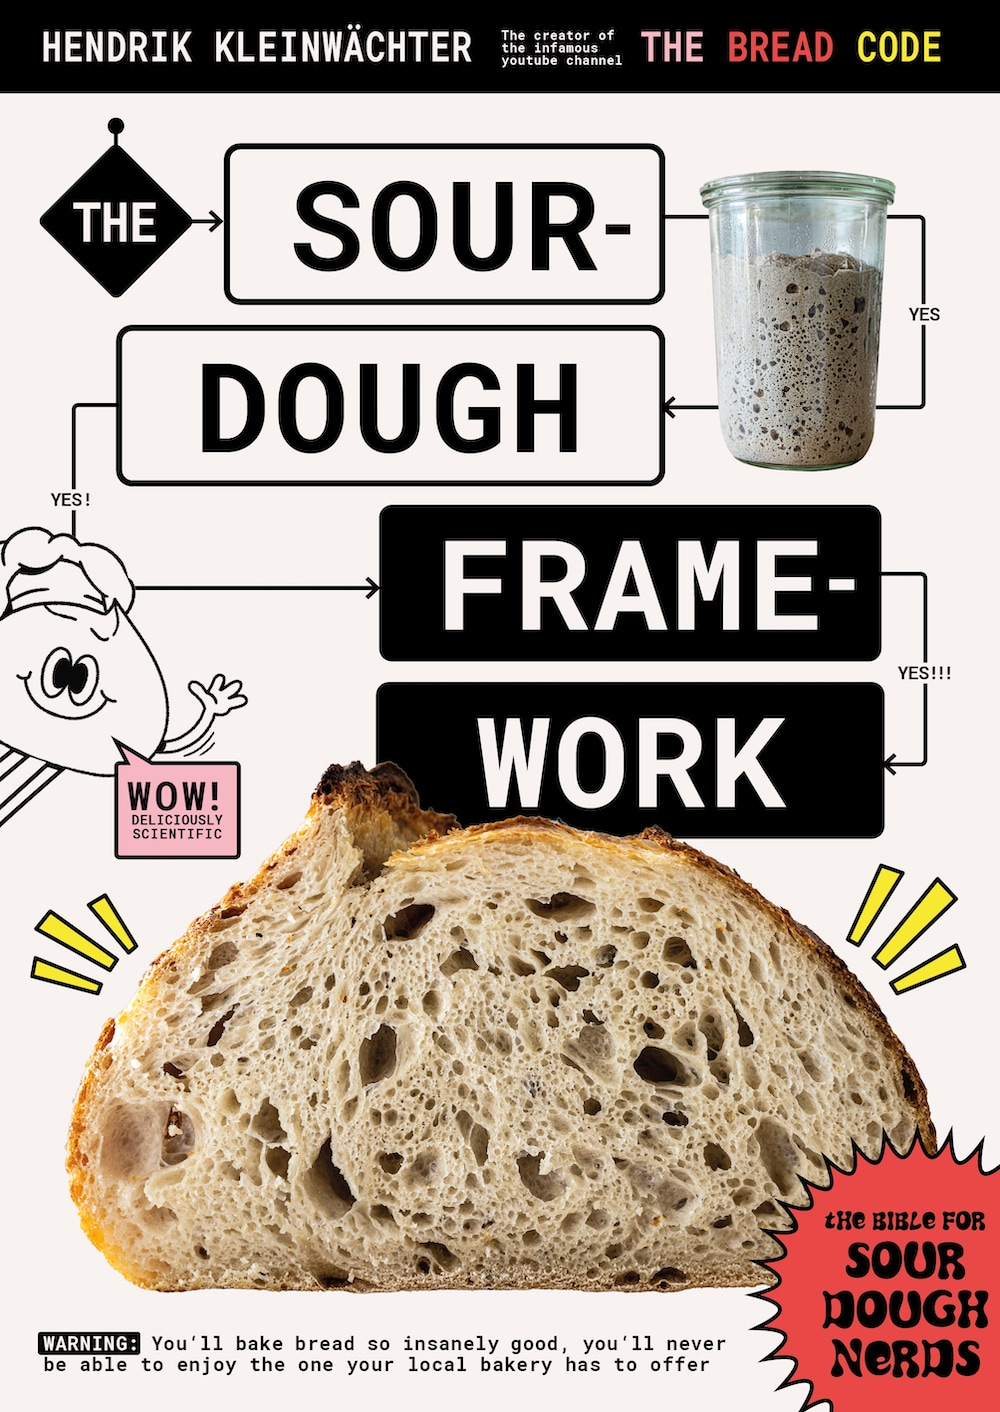
\includegraphics[width=1.33\linewidth]{cover/cover-page.jpg}}
\end{picture}

\newpage
\thispagestyle{empty}

\rule{1pt}{\textheight} % Vertical line
 % Whitespace between the vertical line and title page text
\hspace{0.05\textwidth}
 % Paragraph box for holding the title page text, adjust the width to move the
% title page left or right on the page
%\raggedleft%
\parbox[b]{0.75\textwidth}{%
{\Huge\bfseries The Sourdough Framework}\\[2\baselineskip] % Title
{\large\textit{Version: \today}}\\[4\baselineskip]
{\Large\textsc{Hendrik Kleinwächter}} % Author name, lower case for consistent small caps

% Whitespace between the title block and the copyright text
\vspace{0.5\textheight}

{\noindent The full source code for the book is available at \\
\url{https://github.com/hendricius/the-sourdough-framework/} under CC-BY-SA
license. Do not hesitate to report mistakes or sug\-gestions for
improvements. A hardcover version of the book is also available. More information here:
\url{https://www.breadco.de/hardcover-book}}\\[\baselineskip]
}
